\documentclass[]{article}
\usepackage[UTF8]{ctex}
\usepackage[a4paper,left=10mm,right=10mm,bottom=10mm,top=10mm]{geometry}
\usepackage{graphicx}
\usepackage{float}
\usepackage{amsmath,amsfonts,amssymb,amsthm}
\usepackage{array,color}
%opening
\title{计算机科学中的数学基础Exercise12}
\author{陈昱衡 521021910939}
\date{\today}

\begin{document}

\maketitle
\section*{Warmup10}
\begin{figure}[H]
    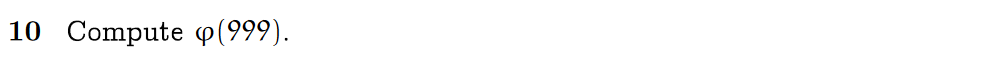
\includegraphics[scale = 0.6]{2023-03-23-10-17-02.png}
\end{figure}
由
\begin{align}
    \varphi(m_1 m_2) &= \varphi(m_1) \varphi(m_2) \text { \quad if  $m_1$ $\perp$ $m_2$}
\end{align}
可知,
\begin{align}
    \varphi(999) &= \varphi(27) \times \varphi(37)\\
    &= 18 \times 36\\
    &=648
\end{align}
或者,也可以由公式(4.53)
\begin{align}
    \varphi(999) &= 999 \times (1-\frac{1}{3})(1-\frac{1}{37})\\
    &=648
\end{align}

\section*{Warmup11}
\begin{figure}[H]
    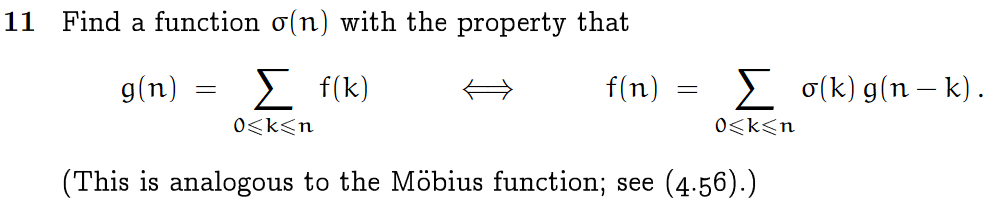
\includegraphics[scale = 0.6]{2023-03-23-10-18-57.png}
\end{figure}
类比于莫比乌斯函数,我们可以得到$\sigma (n)$的如下定义:
\begin{align}
    \sigma (0) = 1 \\
    \sigma (1) = -1\\
\end{align}
代入验证:
\begin{align}
    f(n) &= g(n) - g(n-1)\\
    f(n) &= g(0) \text{\quad if n = 0} \\
\end{align}
则,
\begin{align}
    g(n) &= g(n) - g(n-1) + g(n-1) - g(n-2) + g(n-2) + \cdots + g(1) - g(0) + g(0)\\
    &= \sum_{0 \le k \le n} f(n)
\end{align}



\section*{Warmup12}
\begin{figure}[H]
    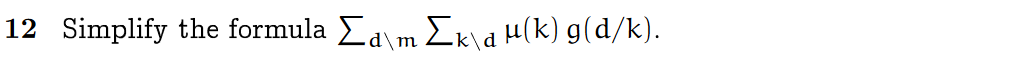
\includegraphics[scale = 0.6]{2023-03-23-10-20-01.png}
\end{figure}
由(4.56),
\begin{equation}
    g(m) = \sum_{d \textbackslash m} f(d) \Leftrightarrow f(m) = \sum_{d \textbackslash m} \mu (d)g(\frac{m}{d}) \\
\end{equation}
有:
\begin{align}
    \sum_{d\textbackslash m}\sum_{k\textbackslash d} \mu (k)g(d/k) &= \sum_{d \textbackslash m}f(k)\\
    &= g(m)
\end{align}


\section*{Warmup13}
\begin{figure}[H]
    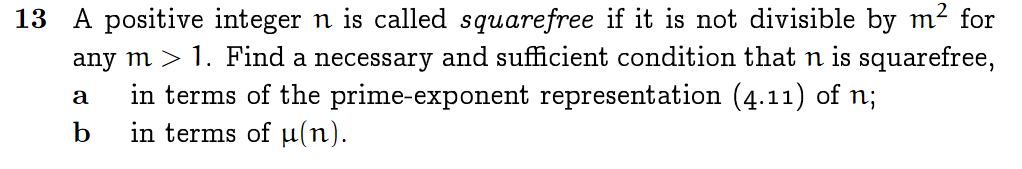
\includegraphics[scale = 0.6]{2023-03-23-10-20-20.png}
\end{figure}

\begin{enumerate}
    \item 由素数幂的定义:
    可知,若$n$不为任何一个$m^2$的整数倍,则其包含的任何一个质数的次数也都不超过两次,因此有:
    \begin{align}
        m_p \le 1
    \end{align}

    \item  由(4.57),
    \begin{align}
        \mu(m) &= \prod \mu (p ^{m_p})\\ 
        & = \left\{
        \begin{array}{l}
            (-1)^r,m=p_1p_2\cdots p_r,\\
            0, p^2 \textbackslash m
        \end{array}
        \right.
    \end{align}
    故,可知,若用$\mu(n)$表示,即为$\mu(n) \neq 0$
\end{enumerate}



\section*{Basics18}
\begin{figure}[H]
    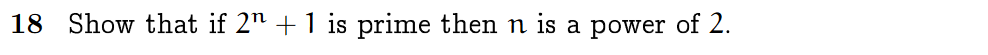
\includegraphics[scale = 0.6]{2023-03-23-10-20-49.png}
\end{figure}
利用反证法,若 $(2^n +1)$ 是素数且$n$不是$2^m$,则,不妨令:
\begin{align}
    n &= km 
    \text{\quad (k is odd)}
\end{align}
则,
\begin{equation}
    2^n = 2^{km} 
\end{equation}
可拆解为:
\begin{align}
    2^{km} &= (2^m + 1) (2^{n-m} - 2^{n-2m} + \cdots - 2^{m} + 1 )
\end{align}

则显然$2^n$ 不是素数。
而若$n=2^m$,则无法拆解为这种形式,
因为
\begin{align}
    (2^{n-m} - 2^{n-2m}  \cdots - 2^{m} + 1) 
\end{align}
有奇数项。

\end{document}